% Common preamble for PIGMIE patent figures (A4).
% Drawing conventions:
%   - A4 portrait
%   - Sans-serif throughout (Helvetica)
%   - "Fig. N" sentence-case caption near top
%   - Page "N/total" at top centre
%   - Reference numerals outside boxes via leader lines
%   - ALL CAPS labels in component boxes
%   - Reactor uses north-east-lines hatched fill
%   - Scene uses double-line border
%   - Module enclosures use dashed line with internal numeral

\documentclass[a4paper,10pt]{article}
\usepackage[top=2.5cm,bottom=1.0cm,left=2.5cm,right=1.5cm]{geometry}
\usepackage[T1]{fontenc}
\usepackage{helvet}
\renewcommand{\familydefault}{\sfdefault}
\usepackage{amsmath,amssymb,bm}
\usepackage{tikz}
\usetikzlibrary{shapes,shapes.geometric,shapes.misc,arrows.meta,positioning,fit,calc,backgrounds,decorations.pathreplacing,decorations.markings,patterns}
\pagestyle{empty}
\setlength{\parindent}{0pt}

\tikzset{
  % Component box: ALL CAPS label inside, no numeral inside
  cbox/.style={draw, rectangle, minimum height=1.0cm, minimum width=2.4cm,
               align=center, line width=0.5pt, font=\small},
  cbox-tall/.style={cbox, minimum height=1.6cm},
  cbox-wide/.style={cbox, minimum width=3.0cm},
  cbox-narrow/.style={cbox, minimum width=1.8cm, font=\footnotesize},
  % Reactor / physical medium: hatched fill
  reactor/.style={cbox, pattern=north east lines, pattern color=black!70},
  % Scene: double-line border
  scenebox/.style={cbox, double, double distance=1.2pt, line width=0.4pt},
  % Module / sub-module enclosure
  enclosure/.style={draw, rectangle, dashed, line width=0.4pt, inner sep=10pt, rounded corners=2pt},
  enclosure-solid/.style={draw, rectangle, line width=0.5pt, inner sep=10pt, rounded corners=2pt},
  % Arrows
  flowarr/.style={-Latex, line width=0.5pt, font=\scriptsize},
  flowbi/.style={Latex-Latex, line width=0.5pt, font=\scriptsize},
  flowarr-fb/.style={-Latex, line width=0.5pt, dashed, font=\scriptsize},
  % Reference numeral leader-line endpoint and label
  refnum/.style={font=\footnotesize, inner sep=1pt},
  leader/.style={line width=0.4pt, -Latex},
  % Caption banner
  figcap/.style={font=\bfseries\large}
}

% Helper: figure header (page number + Fig. N caption)
\newcommand{\figheader}[3]{%
  % #1 = page number (e.g. "1"), #2 = total pages, #3 = figure label (e.g. "1" or "4A")
  \noindent\hfill\small #1/#2\hfill\null\par
  \vspace{0.2cm}
  \begin{center}\bfseries Fig.\ #3\end{center}
  \vspace{0.2cm}
}


\begin{document}

\figheader{3}{3}{3}

\begin{center}
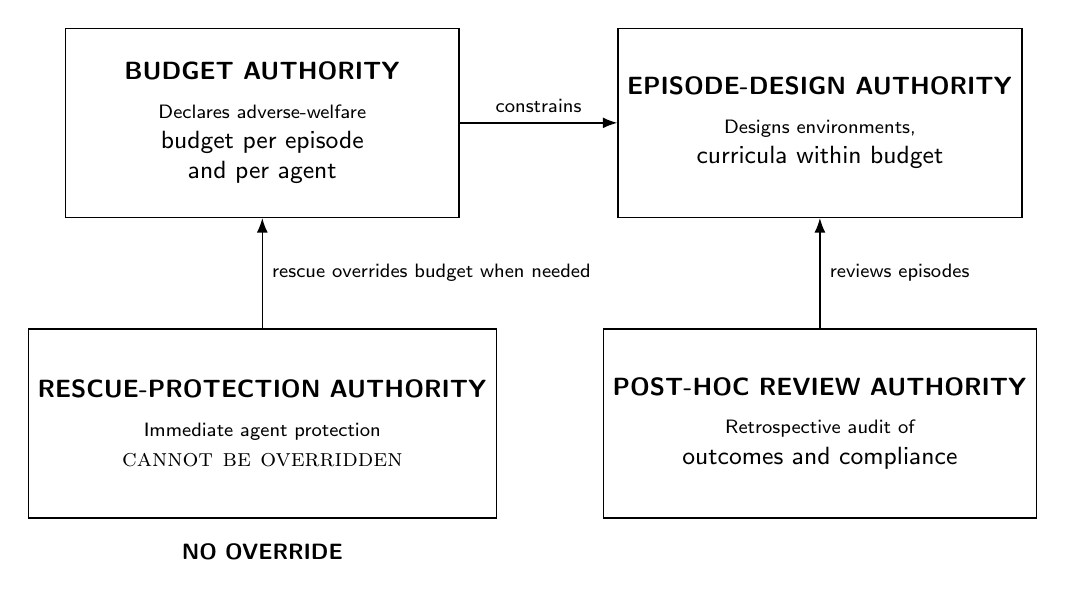
\begin{tikzpicture}[node distance=8mm]

% ============== TOP ROW: Budget + Episode-design ==============
\node[cbox-tall, minimum width=5cm, minimum height=2.4cm, align=center] (budget)
  {\textbf{BUDGET AUTHORITY}\\[3pt]
   \scriptsize Declares adverse-welfare\\budget per episode\\and per agent};
\node[cbox-tall, right=20mm of budget, minimum width=5cm, minimum height=2.4cm, align=center] (episode)
  {\textbf{EPISODE-DESIGN AUTHORITY}\\[3pt]
   \scriptsize Designs environments,\\curricula within budget};

\draw[flowarr] (budget.east) -- node[above] {constrains} (episode.west);

% ============== BOTTOM ROW: Rescue-protection + Post-hoc review ==============
\node[cbox-tall, below=14mm of budget, minimum width=5cm, minimum height=2.4cm, align=center] (rescue)
  {\textbf{RESCUE-PROTECTION AUTHORITY}\\[3pt]
   \scriptsize Immediate agent protection\\\textsc{cannot be overridden}};
\node[cbox-tall, below=14mm of episode, minimum width=5cm, minimum height=2.4cm, align=center] (review)
  {\textbf{POST-HOC REVIEW AUTHORITY}\\[3pt]
   \scriptsize Retrospective audit of\\outcomes and compliance};

\draw[flowarr] (rescue.north) -- node[right, font=\scriptsize] {rescue overrides budget when needed} (budget.south);
\draw[flowarr] (review.north) -- node[right, font=\scriptsize] {reviews episodes} (episode.south);

% NO OVERRIDE annotation under rescue
\node[font=\bfseries\footnotesize, below=2mm of rescue] {NO OVERRIDE};

\end{tikzpicture}
\end{center}

\end{document}
